%%%%%%%%%%%%%%%%%%%
%%% 2025-02-11 %%%%
%%%%%%%%%%%%%%%%%%%
\section{La plataforma ROS (2025-02-11)}
\begin{frame}\frametitle{La plataforma ROS}
  
\includegraphics[width=0.3\textwidth]{Figures/ROS/Ros_logo.png}
  \[\]
  \textbf{ROS (Robot Operating System) } es un \textit{middleware} de código abierto para el desarrollo de robots móviles.
  \begin{itemize}
  \item Implementa funcionalidades comúnmente usadas en el desarrollo de robots como el paso de mensajes entre procesos y la administración de paquetes.
  \item Muchos drivers y algoritmos ya están implementados.
  \item Es una plataforma distribuida de procesos (llamados \textit{nodos}).
  \item Facilita el reuso de código.
  \item Independiente del lenguaje (Python y C++ son los más usados).
  \item Facilita el escalamiento para proyectos de gran escala. 
  \end{itemize}
\end{frame}

\begin{frame}\frametitle{Conceptos}
  ROS se puede entender en dos grandes niveles conceptuales:
  \begin{itemize}
  \item \textbf{Sistema de archivos:} Recursos de ROS en disco
  \item \textbf{Grafo de procesos:} Una red \textit{peer-to-peer} de procesos (llamados nodos) en tiempo de ejecución.
  \end{itemize}
\end{frame}

\begin{frame}\frametitle{Sistema de archivos}
  \begin{columns}
    \begin{column}{0.5\textwidth}
      Recursos en disco:
      \begin{itemize}
      \item \textbf{Workspace:} carpeta que contiene los paquete desarrollados
      \item \textbf{Paquetes:} Principal unidad de organización del software en ROS (concepto heredado de Linux)
      \item \textbf{Manifiesto:} (\texttt{package.xml}) provee metadatos sobre el paquete (dependencias, banderas de compilación, información del desarrollador)
      \item \textbf{Mensajes (msg):} Archivos que definen la estructura de un \textit{mensaje} en ROS.
        \item \textbf{Servicios (srv):} Archivos que definen las estructuras de la petición (\textit{request}) y respuesta (\textit{response}) de un servicio. 
      \end{itemize}
    \end{column}
    \begin{column}{0.4\textwidth}
      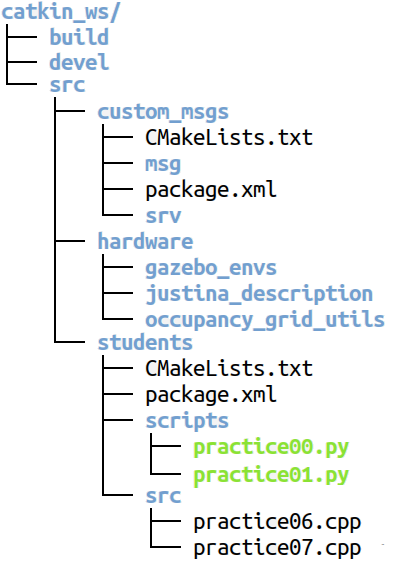
\includegraphics[width=\textwidth]{Figures/ROS/catkin_tree.png}
    \end{column}
  \end{columns}
\end{frame}

\begin{frame}\frametitle{Grafo de procesos}
  El grafo de procesos es una red \textit{peer-to-peer} de programas (nodos) que intercambian información entre sí. Los principales componentes del este grafo son:
  \[\]
  \begin{columns}
    \begin{column}{0.5\textwidth}
      \begin{itemize}
      \item master
      \item servidor de parámetros
      \item nodos
      \item mensajes
      \item servicios 
      \end{itemize}
    \end{column}
    \begin{column}{0.5\textwidth}
      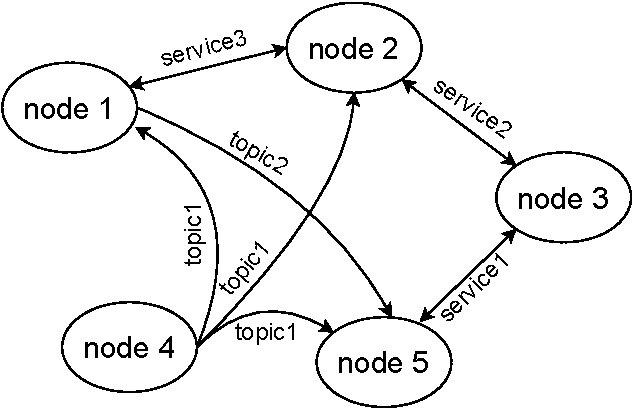
\includegraphics[width=\textwidth]{Figures/ROS/RosGraph.pdf}
    \end{column}
  \end{columns}
\end{frame}

\begin{frame}\frametitle{Tópicos y servicios}
  Los nodos (procesos) en ROS intercambian información a través de dos grandes patrones:
  \begin{columns}
    \begin{column}{0.6\textwidth}
        \begin{itemize}
        \item \textbf{Tópicos}
          \begin{itemize}
          \item Son un patrón $1:n$ de tipo \textit{publicador/suscriptor}
          \item Son no bloqueantes
          \item Utilizan estructuras de datos definidas en archivos \texttt{*.msg} para el envío de información
          \end{itemize}
        \item \textbf{Servicios}
          \begin{itemize}
          \item Son un patrón $1:1$ de tipo \textit{petición/respuesta}
          \item Son bloqueantes
          \item Utilizan estructuras de datos definidas en archivos \texttt{*.srv} para el intercambio de información. 
          \end{itemize}
        \end{itemize}
    \end{column}
    \begin{column}{0.4\textwidth}
      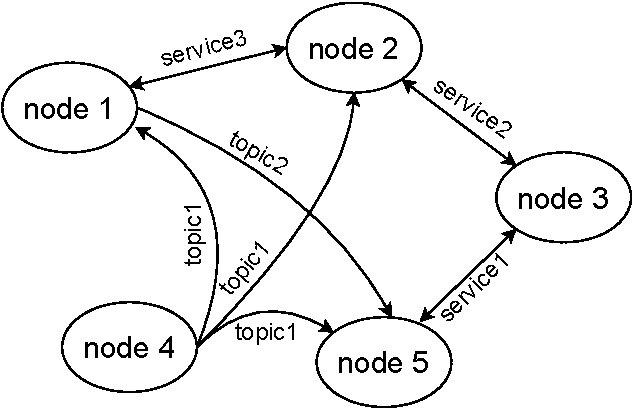
\includegraphics[width=\textwidth]{Figures/ROS/RosGraph.pdf}
    \end{column}
  \end{columns}
  \[\]
  Para mayor información:
  \begin{itemize}
  \item Tutoriales \url{http://wiki.ros.org/ROS/Tutorials}
  \item Koubâa, A. (Ed.). (2020). Robot Operating System (ROS): The Complete Reference. Springer Nature
  \end{itemize}
\end{frame}

\begin{frame}\frametitle{El visualizador RViz}
  \begin{itemize}
  \item Es un nodo de ROS que tiene \textit{plugins} para dibujar en pantalla diversos tipos de mensajes: lidar, mapas, robots, nubes de puntos, rutas, entre muchos otros.
  \item Funciona suscribiéndose a los tópicos indicados por el usuario.
  \item Utiliza el paquete \textit{tf} para dibujar todo con respecto a un sistema de referencia.
  \end{itemize}
  \begin{figure}
    \centering
    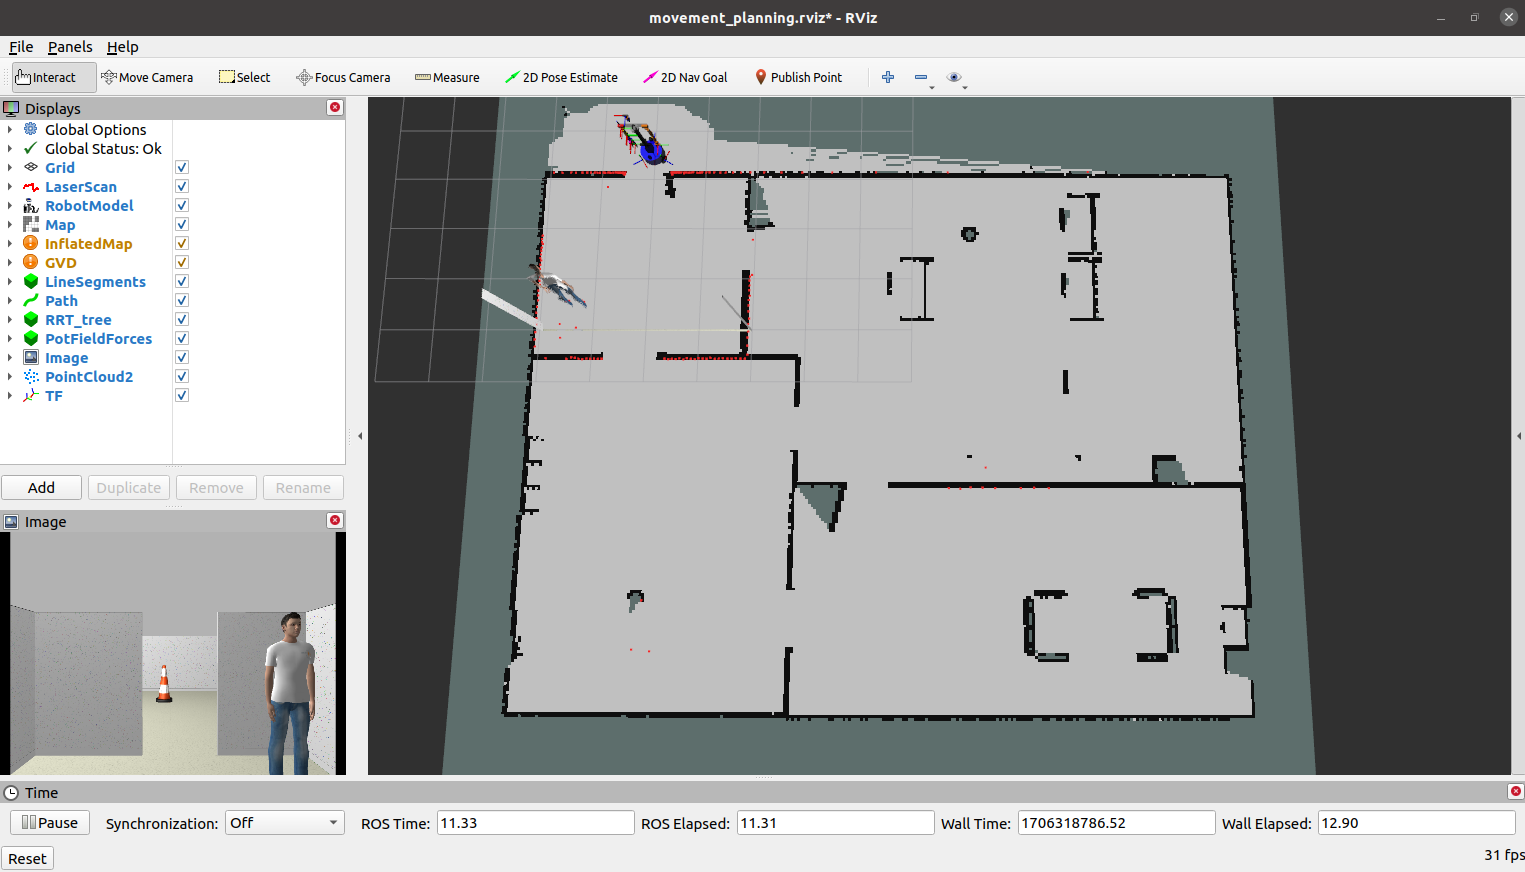
\includegraphics[height=0.5\textheight]{Figures/ROS/rviz.png}
  \end{figure}
\end{frame}

\begin{frame}\frametitle{El simulador Gazebo}
  \begin{itemize}
  \item Acceso a múltiples motores de físicas de alto rendimiento como: ODE, Bullet, Simbody y DART
  \item Existen \textit{plugins} para los sensores y actuadores más comunes en robots móviles (lidar, cámara RGB-D, motores, base diferencial, entre otros)
  \item Los componentes básicos son los \textit{modelos} (archivos \texttt{*.sdf}) y los \textit{mundos} (archivos \texttt{*.world})
  \item Fácil integración con ROS 
  \end{itemize}
  \begin{figure}
    \centering
    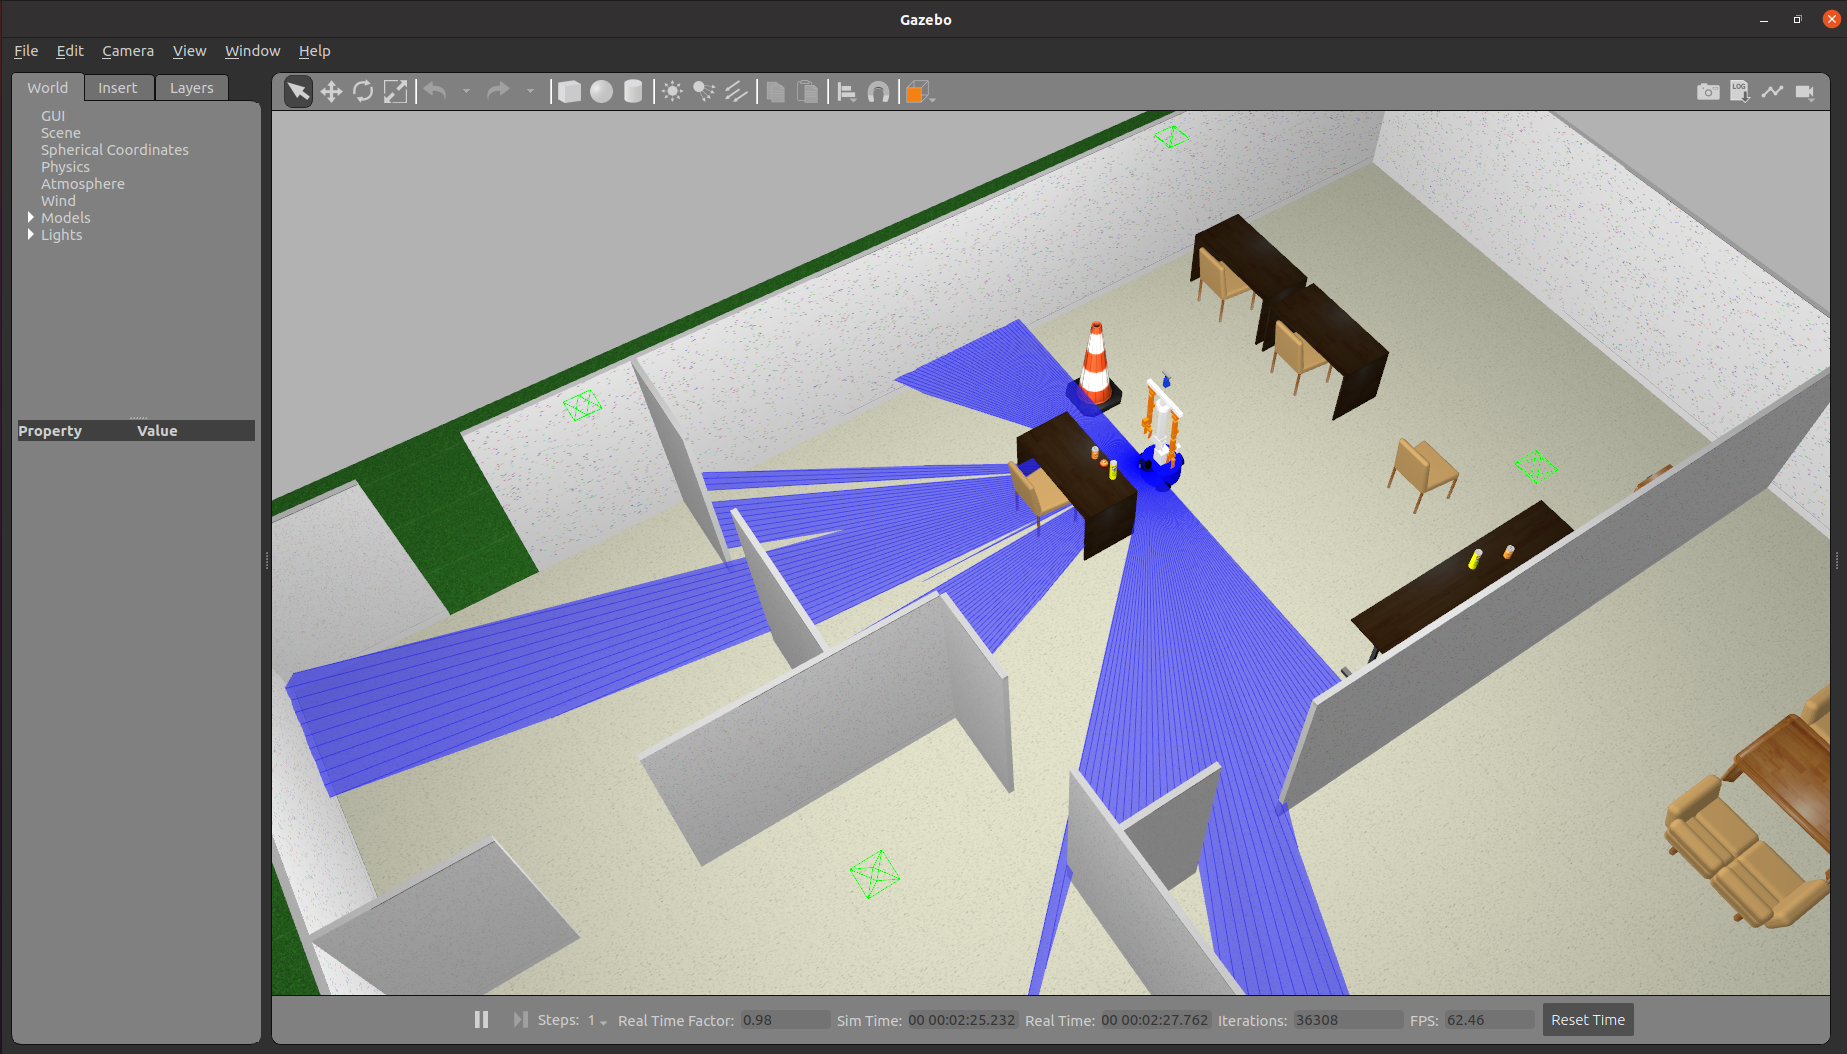
\includegraphics[height=0.6\textheight]{Figures/ROS/gazebo.png}
  \end{figure}
\end{frame}

\begin{frame}[containsverbatim]\frametitle{Tarea 02 - La plataforma ROS}
  Ver instrucciones en Classroom
  \[\]
  \textbf{Deadline: } 2025-02-13 al inicio de la clase. 
\end{frame}


